\documentclass[10pt]{article}

\usepackage{spheric}
%%%TITLE
\title{Numerical study of the mechanism of explosive/impact welding using an improved SPH method}
\date{}

%%AFFILIATIONS
\author[1,2]{M. B. Liu$^\dagger$}
\author[1]{Z. L. Zhang}
\affil[1]{BIC-ESAT, College of Engineering, Peking University, Beijing 100187, China}
\affil[2]{State Key Laboratory for Turbulence and Complex Systems, Peking University, Beijing 100871, China}
\affil[$\relax$]{\email{\dagger}{mbliu@pku.edu.cn}}


%%DOCUMENT
\begin{document}

\maketitle

%\SelectedTopics{}

%%PLEASE PUT YOUR ABSTRACT HERE
\begin{abstract}
Explosive welding (EXW) involves processes like the detonation of explosive, impact of metal structures and strong fluid-structure interaction, while the whole process of explosive welding has not been well modeled before \cite{mousavi2005numerical}. In this paper, a novel smoothed particle hydrodynamics (SPH) model is developed to simulate explosive welding \cite{liu2010smoothed,liu2017density}. In the SPH model, a kernel gradient correction algorithm is used to achieve better computational accuracy. A density adapting technique which can effectively treat large density ratio is also proposed. Typical phenomena in EXW such as the wavy interface, jetting formation, temperature and pressure distribution at the interfaces and melting voids are investigated by the present SPH simulations (shown in Fig. \ref{fig:58-1}, Fig. \ref{fig:58-2} and Fig. \ref{fig:58-3}), which are usually difficult for grid based methods. The mechanisms of wave formation are investigated, specially, two well-known mechanisms namely, the jet indentation mechanism and the vortex shedding mechanism are studied with the present simulations. Based on the well captured interfacial morphologies, the weldability windows for the impact welding (IMW) are given and are compared with the experimental and theoretical results. Furthermore, the weldability windows for EXW with respect to explosive quantity and initial welding angle are obtained. Meanwhile, welding limits and effective explosive quantity for EXW are discussed in detail.


\begin{figure}[!htb]
\begin{minipage}[t]{0.46\linewidth}
\centering
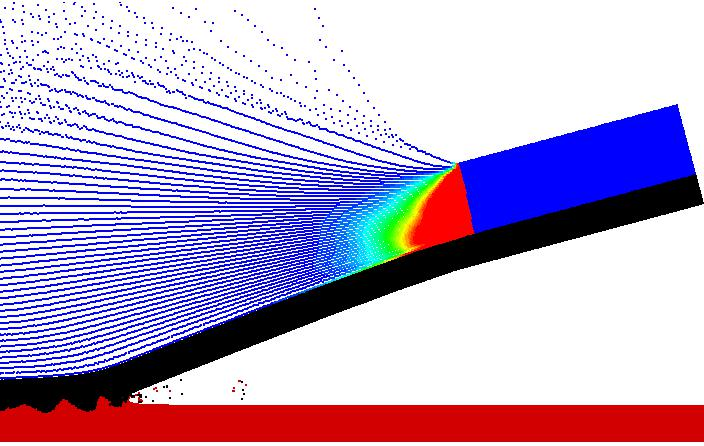
\includegraphics[width=0.8\textwidth]{58-1.png}
\caption{Spread of the explosion wave in the explosives.}\label{fig:58-1}
\end{minipage}
\begin{minipage}[t]{0.05\linewidth}
~~
\end{minipage}
\begin{minipage}[t]{0.46\linewidth}
\centering
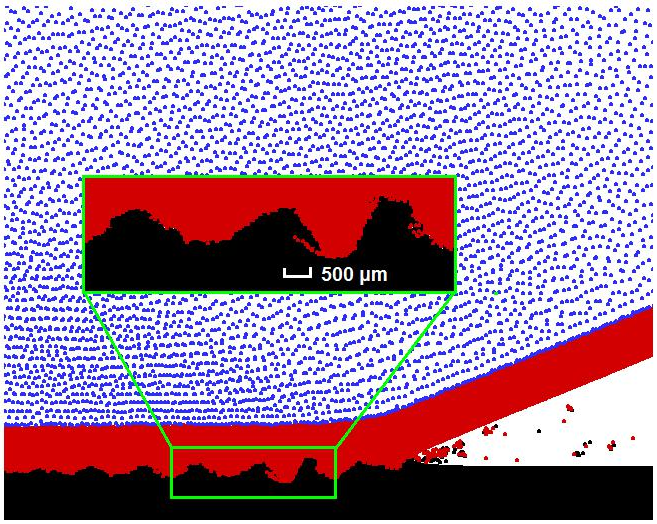
\includegraphics[width=0.7\textwidth]{58-2.png}
\caption{Wavy interface and jetting produced by the EXW.}\label{fig:58-2}
\end{minipage}
\end{figure}

\begin{figure}[!htb]
\centering
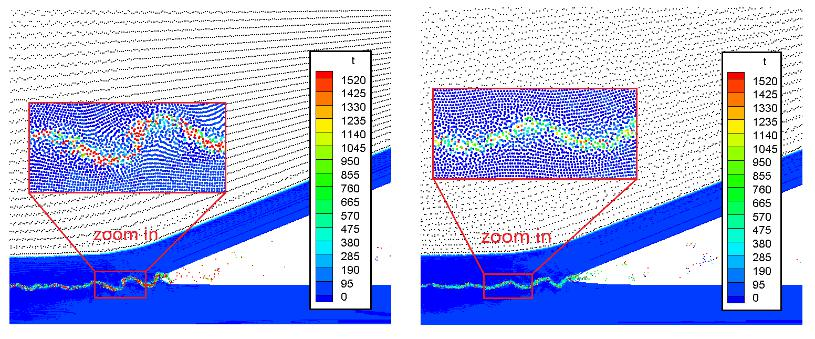
\includegraphics[width=0.7\textwidth]{58-3.png}
\caption{Temperature distribution in EXW with $M_\text{explosive}/M_\text{plate} = 0.1596$ (left) and 0.1915 (right), the welding angle is $15^\circ$.}\label{fig:58-3}
\end{figure}

\end{abstract}


%%THE END OF ABSTRACT

\addbib

\end{document}
